% Drawing 91/07-1 -- folder 91, batch 07, archive page 127 (PDF page 128).
% Transcription: deux flèches descendent de $\mathfrak{X}$ et de $\mathfrak{X}_\xi$ et convergent vers un même point, sans but écrit.
% Kind: two converging arrows. Method 2 (schematic redraw from the facsimile). Status: ok.
% Notes: Two arrows go down from frak X and frak X_xi and converge at one point, with no target written.
% Coordinates: 1 unit = 1 mm = 1/100 of the crop width (bbox in page fractions: [0.1, 0.28, 0.32, 0.42]).
% Redrawn by Claude (claude-opus-5-5), issue #73, 2026-11-07; not checked by a human; not compiled (no TeX in the session).
% Rights: reproduces part of the work -- behind RENDER_TRANSCRIPTS, never published by itself.
\documentclass[tikz,border=3pt]{standalone}
\usepackage{amsmath,amssymb}
\usetikzlibrary{patterns,arrows.meta}
\tikzset{pencil/.style={black!45}, struck/.style={black!35}, mark/.style={circle,draw,inner sep=1.3pt}, pt/.style={circle,fill,inner sep=0.9pt}, opt/.style={circle,draw,fill=white,inner sep=1.1pt}}
\begin{document}
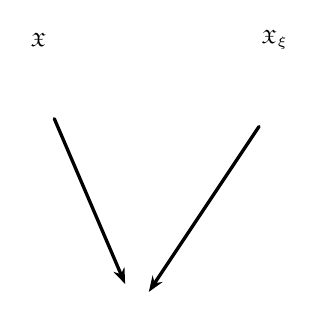
\begin{tikzpicture}[x=1mm,y=1mm,line cap=round,line join=round,font=\scriptsize]
\node[inner sep=1pt] at (38,-26) {\scriptsize $\mathfrak X$};
\node[inner sep=1pt] at (68,-26) {\scriptsize $\mathfrak X_\xi$};
\draw[-{Stealth[length=2mm]},very thick] (40,-36) -- (49,-57);
\draw[-{Stealth[length=2mm]},very thick] (66,-37) -- (52,-58);
\end{tikzpicture}
\end{document}
